
\chapter{Preface}
\todo[inline]{The preface has to be more detailed}

Recent years have seen significant increases in the scope and complexity of digital systems - cf. hhe uprise of Cyber-Physical Systems. Developers, providers, and users have recognized the necessity to devote greater attention to the adoption of innovative technologies. It requires a novel type of preparedness, in particular to the process of design and dynamic adaptation to emergent systems. Since subject-oriented thinking and design supports a human-oriented way to structure and imoplement complex systems, its approach to modeling and execution should be 'standardized', as different teams or modelers could interpret subject oriented means of representation differently. Since subject-orientation is a behavior-centered approach to system understanding and development, non-standardized application could easily lead to non-intended behavior of systems or their components.

However, standardization efforts requires essential steps, among them (see also Figure \ref{fig:Standardisation_Process} )the process into seven steps.


\begin{figure}[h]
	\centering
	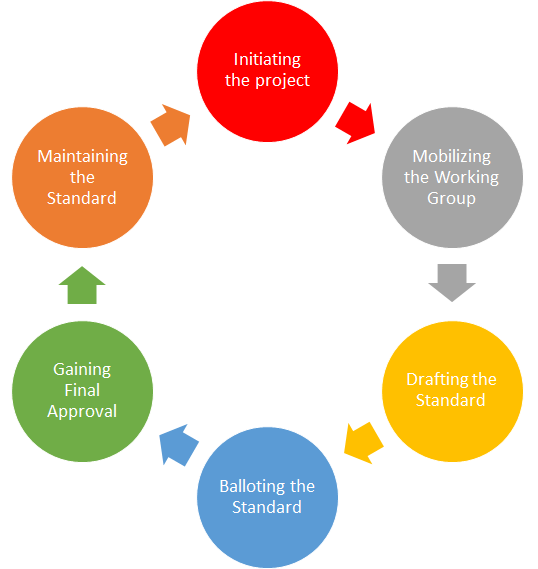
\includegraphics[width=0.7\linewidth]{Figures/Preface}
	\caption[Standardisation Process]{Standardisation Process}
	\label{fig:Standardisation_Process}
\end{figure}


\begin{enumerate}
	\item initiating the project

Although we have started in 2012 (Fleischmann et al., 2012) the needs for a standard has been identified 2 years ago. We started documenting (Referenz zu paper bei S-BPM 2019?) experiences from providers, users, researchers and system developers. Technological advancements in model execution have led to standardize the semantics, in order to reflect the novel opportunities. Once a need is identified, a proposal to create a new standard has to be put forward.

 \item  Mobilize a working group

Standards are created or reviewed by experts in the relevant field. They include researchers, providers, users and communities of practice, who form into a some technical committee, termed the Standardization Gang for subject orientation.

\item Balloting the standard by public review 

The technical committee conducts preliminary research and creates a draft outline of the new standard. Much of this initial work can be done remotely or in sub groups, however, needs to be consolidated at some point in time. This is where we are today when providing this edition of consolidated standard inputs.

\item Gain approval 

Once a draft is written, it requires approval for public review. This consensus is required in order to progress any further. The next step is to include all feedback and create a revised document for final public review. Thereby, anyone is welcome to provide feedback to improve the quality and ensure all relevant areas and perspectives are captured.

\item Publish and Maintain 

After public review, the standard goes back to the technical committee to make amendments it deems necessary based on the feedback received. The committee then approves the final version of the standard. After the revised standard receives that final approval from the technical committee, it is officially released. System developers or providers may incorporate it into their practice.

\end{enumerate}


The current version is intended for researcher who work in the area of software engineering and business process management. It helps understanding the approach through in-depth provision of the practical and theoretical aspects of subject oriented modeling and implementing systems.\\
The book is a collection of all the essential aspects of subject oriented modeling and programming. Many parts of this documents are reprints of various books and papers. Table \ref{tbl:sources} shows the sources for the various chapters and sections.\\
In chapter 1 an overview is given to the subject orientated language PASS and the methods which are used to describe its structural and execution semantics. OWl (Web Ontology Language) \cite{Web:OWL} is used to describe the structural semantics and Abstract State Machines (ASM) \cite{book:ASM-2018}, \cite{book:ASM-2003} is applied to specify the execution demantics precisely.\\
In chapter 2 the structure of PASS specification is considered in detail and its semantic is defined precisely in a formal way using OWL and ASM. The semantic of the execution of PASS models is described in chapter 3. The execution semantic uses coreASM which is an executable extension of the ASM method. This means that models described in PASS can be executed by a coresponding interpreter.\\
Chapter 4 shows how the abstract implementation independent PASS models can be implemented using software components, physical components or human.  A formal language is described how the right ressources are assigned to the entities of the model.\\
In the last chapter some additional aspects of the subject oriented modeling approach is considered. Thes aspects extend the kernel which was defined in chapter 2, 3 and 4.\\
The appendix contains the details of the formal semantic of PASS. Appendix A contains the complete Ontology, Abbendix B defines the mapping of the ontology to the ASM definition of PASS and Appendix C containes the complete formal execution semantics.



%\begin{longtable}
%	\footnotesize
%	\centering
%	\begin{tabular}[t]{@{}1 p{0.3\linewidth} p{0.3\linewidth} p{0.4\linewidth} @{}}
\todo[inline]{contact publisher for clarifying copyrights}
	\begin{longtable}[t]{ p{1 cm} p{4 cm} p{7 cm} }	
	\toprule
		\textbf{Chapter Nr.} & \textbf{Chapter title}  & \textbf{Source}
		\\
		\midrule
		1.1 \newline 2.1 \newline 3.1 & Subject Orientation and PASS \newline Informal Description \newline Informal Description of Subject Behaviour and its Execution & Fleischmann, Albert; Schmidt, Werner; Stary, Christian; Obermeier, Stefan; B\"orger, Egon; \newline \textit{Subject-Oriented Business Process Management,} \newline Springer Verlag Berlin 2012
		\\
		\midrule
		3.3 & ASM Definition of Subject Execution & 
		\\
		\midrule
		4.1 & People and Organisations & Fleischmann, Albert; Oppl, Stefan; Schmidt, Werner; Stary, Christian;\newline \textit{Contextual Process Digitalization: Changing Perspectives - Design Thinking - Value-Led Design} \newline Springer Verlag Berlin 2020
		\\
		\midrule
		5.1 & Subjects and Shared Input Pools & Fleischmann, A.; Stary, C.,\newline
			\textit{Dependable Data Sharing in Dynamic IoT-Systems - Subject-oriented Process Design, Complex Event Processing, and Blockchains;} \newline
			in Proceedings of S-BPM ONE 2019, 11th International Conference on Subject Oriented Business Process Management,\newline
			editors: Betz, S.;Elstermann, M.; Lederer, M; \newline
			ICPC published by Association of Computing Machinery (ACM) Digital Library; 2019
		\\
		\midrule
		5.2 & Subject-Phase Model based process specifications &  Fleischmann, A.,\newline
		\textit{Activity-Based Costing for S-BPM,}\newline
		Proceedings of the 5th International Conference S-BPM ONE 2013, Computer and Information Sciences (CCIS), No. 360,\newline
		editors: Fischer, H. and Schneeberger, J.\newline
		Springer 2013,
		\\
		\midrule
		5.3 & Hierarchies in Communication Oriented Business Process Models & Elstermann, M and Fleischmann, A.,\newline
		\textit{Modeling Complex Process Systems with Subject Oriebted Means,}\newline
		in Proceedings of S-BPM ONE 2019, 11th International Conference on Subject Oriented Business Process Management,\newline
		editors: Betz, S.;Elstermann, M.; Lederer, M; \newline
		ICPC published by Association of Computing Machinery (ACM) Digital Library; 2019
		\\
		\midrule
		5.4 & Business Activity Monitoring for S-BPM & Schmidt, W.; Fleischmann, A.;\newline
		\textit{Business Process Monitoring with S-BPM,}\newline
		Proceedings of the 5th International Conference S-BPM ONE 2013, Computer and Information Sciences (CCIS), No. 360,\newline
		editors: Fischer, H. and Schneeberger, J.\newline
		Springer 2013,
		\\
		\midrule
		5.5 & Subject Oriented Project Management & Albert Fleischmann, Werner Schmidt, Christian Stary;\newline
		\textit{Subject Oriented Project Management,}\newline
		published in SEAA '14: Proceedings of the 2014 40th EUROMICRO Conference on Software Engineering and Advanced Applications,\newline
		IEEE Computer Society, 2014
		\\
		\midrule
		5.6 & Subject Oriented Fog Computing & Stary, C. ; Fleischmann, A. ; Schmidt, W., \newline
		\textit{Subject-oriented Fog Computing: Enabling Stakeholder Participation in Development,} \newline
		Proceedings of the 4th IEEE World Forum on Internet of Things (WF-IoT), Singapure \newline
		IEEE Xplore Digital Library, DOI 10.1109/WF-IoT.2018.8355167, 2018
		\\
		\midrule
		5.6 & Activity Based Costeing &  Zehbold, C.; Schmidt, W.; Fleischmann, A.,\newline
		\textit{Activity-Based Costing for S-BPM,}\newline
		Proceedings of the 5th International Conference S-BPM ONE 2013, Computer and Information Sciences (CCIS), No. 360,\newline
		editors: Fischer, H. and Schneeberger, J.\newline
		Springer 2013,
		\\
\bottomrule
%\end{tabular}
\caption{Main sources of the various chapters and sections}
\label{tbl:sources}
\end{longtable}